El teorema de Thevenin establece que cualquier circuito eléctrico lineal que
contenga fuentes de voltaje, corriente y resistencias puede ser reemplazado, entre
un par de terminales {\bf a} y {\bf b}, por un circuito equivalente de voltaje $V_{eq}$ y
resistencia en serie $R_{eq}$. Este hecho permite, en esencia, simplificar circuitos
complejos cuyos parámetros son dificiles de deducir analíticamente.

Es posible determinar los parámetros equivalentes de un circuito utilizando un elemento
externo capaz de extraer una cantidad de corriente $I$, p.ej. una resistencia variable
$R_z$. En la Fig. ? se muestra la configuración ideal para medir $V_{eq}$ y $R_{eq}$
utilizando $R_z$ como parámetro.
\begin{figure}[H]
	\centering
	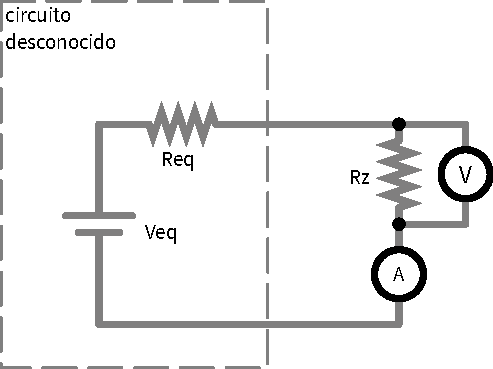
\includegraphics[width=0.9\linewidth]{res/C1.pdf}
	\caption{Configuración para medir el voltaje y resistencia equivalente de un
			circuito desconocido.}
	\label{fig:c1}
\end{figure}